\documentclass[a4paper,11pt]{article}
\usepackage[T1]{fontenc}
\usepackage[utf8]{inputenc}
\usepackage{lmodern}
\usepackage{hyperref}
\usepackage{graphicx}
\usepackage{rotating}
\usepackage{listings}
\usepackage{color}

% Swedish
\usepackage[swedish]{babel}

% Table of contents depth 3 levels: A.B.C
\setcounter{tocdepth}{3}

\begin{document}

\title{Sommarstugekoll \\
	Digital Konstruktion EDA234 \\ Grupp 2}
\author{Names \\
   Chalmers Tekniska Högskola \\
   \texttt{email addresses}}

\maketitle

\pagebreak

\tableofcontents

\pagebreak

\begin{abstract}

	Systemet som beskrivs i denna rapport är ett automatiserat temperaturkontrollsystem som är åtkomstbart och styrbart via
	telefon (DTMF). Systemets huvudfunktionalitet är att informera användaren om de aktuella temperaturerna som läses från
	två anslutna temperatursensorer, och att ge användaren möjlighet att på avstånd styra (av/på) ett antal externa funktioner,
	såsom exempelvis värmeelement. Information och kontrolldata utbytes genom en vanlig analog telefonlinje, med hjälp av DTMF:
	Dual Tone Multiple Frequency. 

	Ett särskilt exempel på användningsområde är kontroll av uppvärmningen i en sommarstuga. Med hjälp av systemet kan man
	undvika att temperaturen sjunker under en viss gräns, vilket skulle kunna få konsekvenser såsom att rör fryser. Genom att
	hålla temperaturen på en lämplig nivå kan man undvika oönskade konsekvenser samtidigt som man minimerar uppvärmningskostnader.
	'Sommarstugekoll' löser detta problem genom att erbjuda ett enkelt sätt att hålla koll på och kontrollera inom- och utomhustemperaturer.
	Om ägaren till en sommarstuga vill göra ett besök ringer han/hon helt enkelt upp sommarstugan och slår på lämpliga element, så att
	sommarstugan hinner värmas till en behaglig temperatur medans ägaren kör dit.

	Systemet självt kräver endast en telefonlinje och en vanlig spänningskälla på 5V. Eftersom det är effektsnålt kan systemet stå
	på under långa perioder, vilket gör det en lätt och trevlig lösning på alla dina sommarstugeuppvärmningsproblem.

\end{abstract}

\section{Introduktion}

\section{Systemspecifikation}

	\begin{tabular}{ l r}
	   Matningsspänning & +5V\\
	   Strömförbrukning & ~80mA\\
	   Någonting & Någonting\\
	\end{tabular}

\section{Systembeskrivning}

\section{Blockschema}

	\begin{figure}[h!]
	  \centering
	      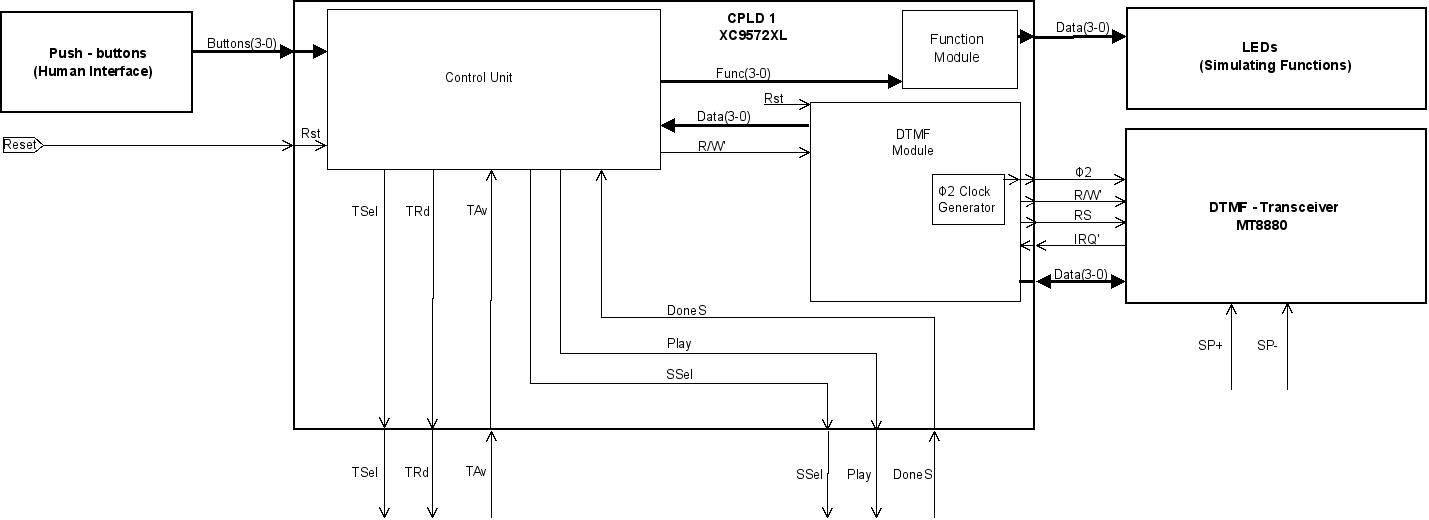
\includegraphics[scale=0.48, angle=90]{BlockDiagramCPLD1.jpg}
	  	\caption{Blockschema (CPLD1)}
	\end{figure}

	\begin{figure}[h!]
	  \centering
	      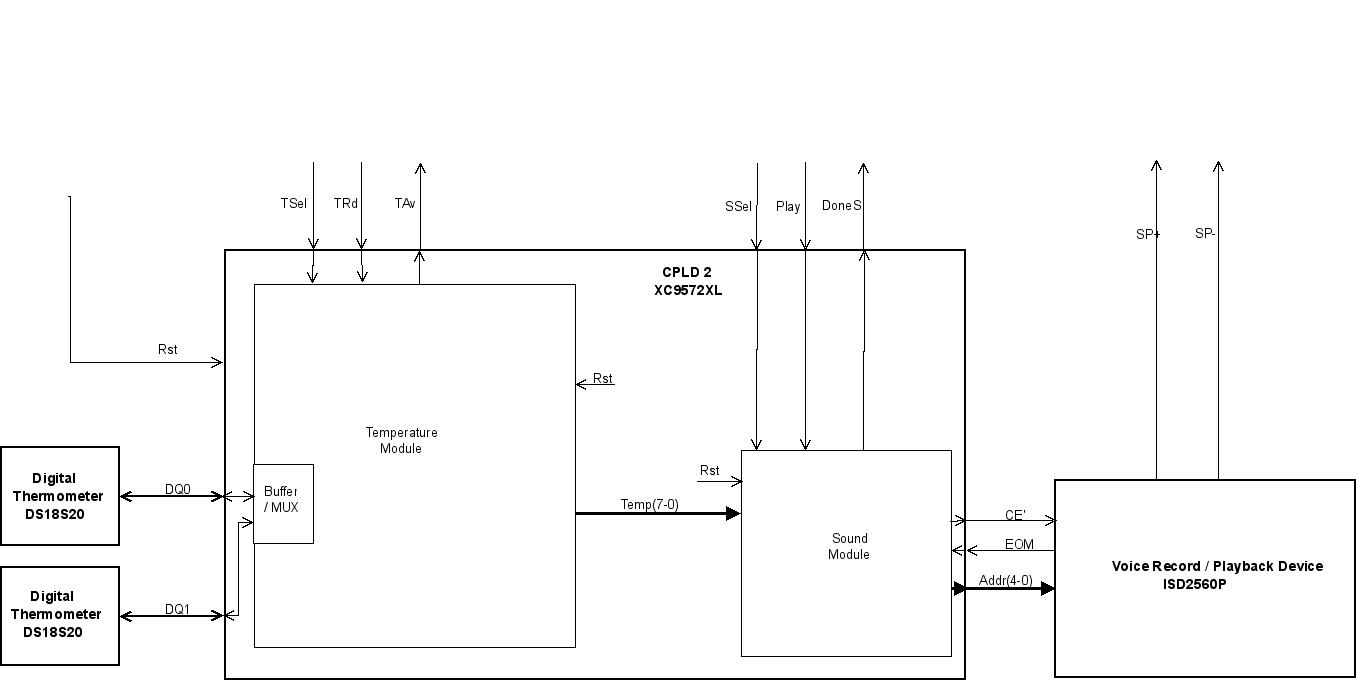
\includegraphics[scale=0.48, angle=90]{BlockDiagramCPLD2.jpg}
	  	\caption{Blockschema (CPLD2)}
	\end{figure}


\section{Block, Funktionalitet}

	\subsection{Dataväg}

	\subsection{Styrenhet}

	\subsection{Funktionsmoduler}

		\subsubsection{DTMF-Modul och MT8880}
	
		\subsubsection{Ljudmodul och ISD2560P}

		\subsubsection{Temperaturmodul och DS18S20}

{\bf Syfte}

Temperaturmodulen i CPLD'n är ansvarig för att hantera seriekommunikationen med 
DS18S20-temperatursensorerna, via entrådsbussarna, samt att ge ut de lästa temperaturerna
i tecken-belopp-format till ljudmodulen, i syfte att låta den i sin tur spela upp de avlästa
temperaturen för systemanvändaren.\\

{\noindent \bf 1-Trådsbuss}

Entrådsbussarna är anslutna till matningsspänning (+5V) genom ett pull-up-motstånd på 4.7kO, och
ändarna av bussen är anslutna till mastern (CPLD) och sensorn (DS18S20), respektive. Då bussen
befinner sig i viloläge dras den hög ("svag drivning") av pull-up-motståndet. När information
skickas över bussen drar den kommunicerande (sändande) enheten bussen låg genom att driva den
med en stark logisk nolla.\\

	\begin{figure}[h!tb]
	  \centering
	      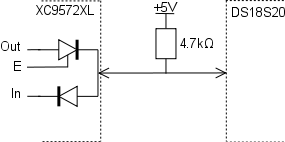
\includegraphics[scale=1, angle=0]{TempBus.png}
	  	\caption{Uppkoppling, Entrådsbuss}
	\end{figure}

{\noindent \bf DS18S20}

Den temperatursensor som används är Maxim DS18S20, som ger temperaturmodulen möjlighet att läsa av temperaturen
med nio (9) bitars upplösning. Sensorerna som användas i detta system drivs av en extern spänningskälla på +5V,
och kommunicerar seriellt över en entrådsbuss. Seriekommunikationen baserar på att bus-mastern initierar skriv-
och läs-luckor. Varje sådan lucka är mellan 60 och 120 us lång. Temperatursensorn initieras genom att mastern
driver bussen låg i åtminstone 480 us, vilket följs av att temperatursensorkretsen själv drar bussen låg i 60-240 us,
efter en återhämtningslucka på minst 1 us. Efter initieringen väntar sensorkretsen på ett ROM-kommando från mastern,
följt av ett Funktions-kommando. Varje sådant kommando är en byte lång, och skickas som LSB-först. Mastern skickar
en logisk nolla genom att driva bussen låg under hela skrivluckan. En etta skickas genom att mastern driver bussen låg
under en kort period, 1-15us, och sedan släpper bussen under resten av skrivluckans längd. Mellan varje skriv- eller läslucka
måste det finnas en återhämtningsperiod på minst 1us.

Då mastern är klar med att skicka över ROM- och Funktions-kommando, kan (beroende på vilka kommandon som sändes) DS18S20-kretsen
svara med aktuell data. På samma sätt som ovan måste mastern här initiera en läs-lucka genom att driva bussen låg i 1-8us, och
sedan släppa den (högimpediv). DS18S20-kretsen svarar på den allokerade läs-luckan genom att antingen hålla bussen låg för att
överföra en nolla, eller genom att låta bussen dras hög av pull-up-motståndet för en etta. Under den här tiden (upp till 15 us
efter att ha släppt bussen) kan mastern sampla bussen för att läsa av vad DS18S20-kretsen skickat. All data som skickas från
temperatursensorn skickas som LSB-först, och i 2-komplementsform.\\

{\noindent \bf Läscykel, Sammanfattning}

En läscykel består av fyra steg: Initialisering, Kommandon, Läsning och Viloläge.

Initialiseringen består i av att mastern driver bussen låg i 512 us, sedan släpper den.
Temperatursensorn svarar med en närvaro-puls genom att driva bussen låg i 106 us, och därgenom bekräftar den sin närvaro
på bussen och sin operationella status.

Då mastern detekterat närvaropulsen börjar den överföra ett ROM-kommando (Skip ROM, 0xCC), följt av en kort återhämtningslucka
och sedan ett Funktions-kommando (Convert Temperature, 0x44), enligt läs-/skriv-luckemetoden som beskrivits ovan.
Skip-ROM-kommandot används i det här systemet eftersom endast en temperatursensor används per entrådsbuss.
Därmed finns inget behov av att kunna addressera specifika sensorer på bussen.
Convert Temperature-kommandot säger till DS18S20-kretsen att börja konvertera temperaturen, och sedan spara den 
lästa temperaturen i sitt interna minne för att sedan läsas av mastern.
Under konverteringsperioden (upp till 750 ms) kan mastern polla temperatursensorns status genom att kontinuerligt
sända förfrågningar genom att dra bussen låg i en kort period (4 us). Temperatursensorn svarar med en nolla
sålänge den är upptagen med att konvertera temperatur, och sedan en etta såfort den är klar.
Då mastern ser att temperatursensorn är klar, initiseras temperatursensorn om och ytterligare ett ROM-Funktions-kommandopar
överförs. Dessa är 0xCC (Skip ROM) följt av 0xBE (Read Scratchpad), respektive.
Idealt ska temperatursensorkretsen nu vara redo att överföra temperaturdata till mastern från sitt interna 9-bytesminne.
Då den ges Read Scratchpad-kommandot börjar DS18S20 sända över innehållet i sitt minne över bussen.
Mastern går då in i läsningsläget och börjar sampla datan på bussen genom att driva bussen låg, släppa den och sampla efter 4 us,
allt enligt den metod som beskrivs ovan. Mastern samplar de första åtta bitarna data som sänds av DS18S20, sedan en ytterligare,
nionde bit. Den sista biten utgör en tecken-bit, 0 för positiv temperatur och 1 för negativ. Då den nionde biten data lästs
ger mastern på nytt en initieringspuls, som säger åt temperatursensorn att sluta sända data.
Den nyligen lästa temperaturen placeras av temperaturmodulen i CPLD'n (på CPLD2) på den interna temperaturbussen, och
TAv sätts till 1 för att indikera att det finns korrekt data på bussen, enligt vad som efterfrågades av styrenheten.\\

	\begin{figure}[h!tb]
	  \centering
	      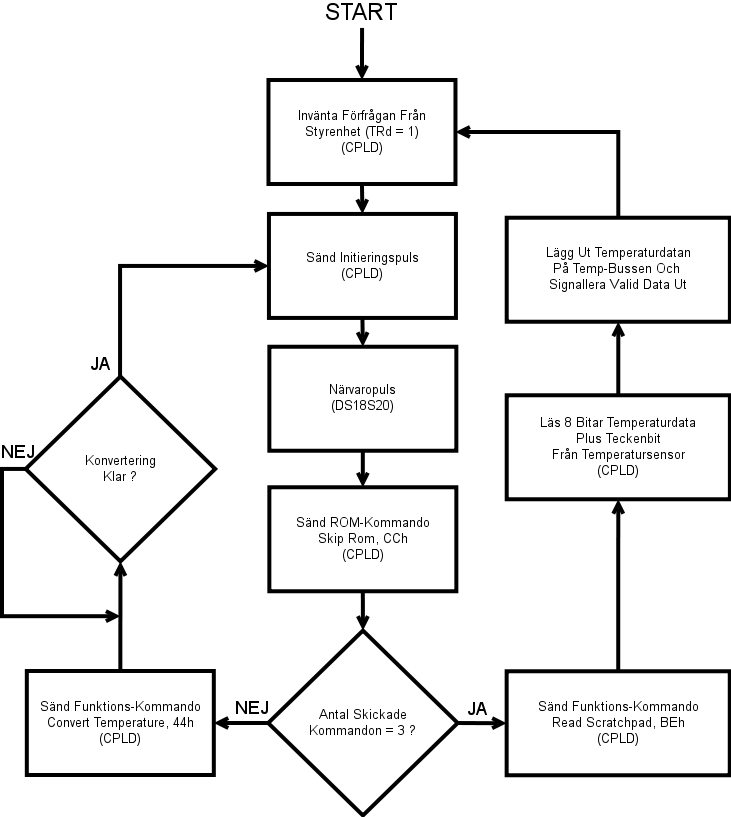
\includegraphics[scale=0.5, angle=0]{ReadCycleFlowChart.png}
	  	\caption{Högnivå-flödesdiagram för Temperaturläscykel}
	\end{figure}

{\noindent \bf Signaler}

	\begin{tabular}{l r}
		\\{\bf In} &  \\
		DQ0 & Kommunikationstråd till temperatursensor 0\\
		DQ1 & Kommunikationstråd till temperatursensor 1\\
		TRd & Styrsignal från styrenheten: Signalerar att läscykel ska inledas\\
		TSel & Styrsignal från styrenheten som väljer temperatursensor (0/1)\\\\
		{\bf Ut} &  \\
		TAv & Signal till styrenheten för att signalera att valid data finns på bussen\\
		Temp & Den interna temperaturdatabussen till ljudmodulen\\\\
	\end{tabular}

{\noindent \bf Detaljer}

Temperaturmodulen är baserad runt en tillståndsmaskin, understödd av en intern Buffer/MUX-modul samt 
ett antal interna räknare för att generera de nödvändiga tidsfördröjningspulserna.\\

{\noindent \bf Buffer/MUX}

Buffer/MUX-modulen är direkt ansluten till de två DS18S20-Temperatursensorerna som använder entrådsbusskommunikationen.
Multiplexern (MUX) används för att välja mellan vilken av de två sensorerna (Sesnor 0 eller Sensor 1) som styrenheten
vill kommunicera med, och använder signalen TSel.
Buffern är en tri-state-buffer med en Enable-signal, E. När E är satt till 1 så kan mastern använda den av TSel valda
entrådsbussen som en utgång för att överföra kommandon. När E är satt till 0 kan mastern läsa data från bussen.\\

{\noindent \bf Räknare}

Internt använder temperaturmodulen ett antal olika räknare: \\
	\begin{tabular}{l c r}
		\\{\bf Namn} & {\bf Bitar} & {\bf Syfte}\\
		cntInt & 9 & Genererar timing-pulser\\
		ZC & 4 & Hanterar timing för skriv-luckor\\
		Progress & 2 & Anger aktuellt kommando (0-3)\\
		bitCnt & 8 & Anger aktuell bit för överföring/läsning\\\\
	\end{tabular}

{\noindent \bf Tillståndsmaskin}

För en uttömmande beskrivning av den interna tillståndsmaskinen som används av temperaturmodulen,
se sektionen om tillståndsmaskiner.\\

		\subsubsection{Kontrollfunktioner}

		\subsubsection{Gränssnitt och Knappar}

\section{Tillståndsmaskiner}
		\subsubsection{DS18S20 Seriell Kommunikation}
			\\(Refererar till tillståndsdiagramet för temperaturmodulen)\\
			{\bf Reset:} Alla signaler och räknare återställs till sina grundvärden.\\
			{\bf Grundvärden:} Utgångspunkten är att alla signaler behåller sina gamla värden om inget annat anges.\\
			\begin{tabular}{l r}
				\\{\bf Initialisering (Tillstånd 0-3):} &  \\
				0 & Viloläge och återställningspunkt. Temperaturmodulen väntar i en slinga tills dess att den detekterar en logisk etta på TRd (Läs temperatur). Vid TRd = 1 börjar tillståndsmaskinen ticka, och sätter TAv = 0, eftersom läscykeln har börjat och den data som finns på temperaturbussen inte längre är valid.\\
				1 & Fördröjningstillstånd, väntar på puls på DelayLong (512 us), går sedan till tillstånd 2.\\
				2 & Mastern driver bussen låg i 512 us och sätter datavärdet till 0xCC (Skip ROM), går sedan till tillstånd 3.\\
				3 & Mastern släpper bussen, vilket tillåter DS18S20 att skicka tillbaka en närvaropuls. Väntar 512 us.\\\\
				{\bf Kommandoöverföring (Tillstånd 4-8):} &  \\
				4 & Förberedelsetillstånd, mastern förbereder sig på att sända och går till tillstånd 5 efter 16 us.\\
				5 & Huvudsändningstillståndet, mastern avgör vilken bit som ska skickas och skickar den (enligt bitCnt-räknaren).\\
				6 & Mellanbittillstånd, återhämtningstillständ. Avgör om det finns fler bitar att skicka i nuvarande byte. Annars fortsätt.\\
				7 & Avgör om DS18S20 är upptagen med att konvertera temperaturen.\\\\
			\end{tabular}

	\begin{figure}[h!tb]
	  \centering
	      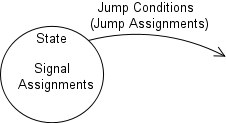
\includegraphics[scale=0.5, angle=0]{StateMachineExplained.png}
	  	\caption{Förklaring till State Machine-diagram}
	\end{figure}

	\begin{figure}[h!tb]
	  \centering
	      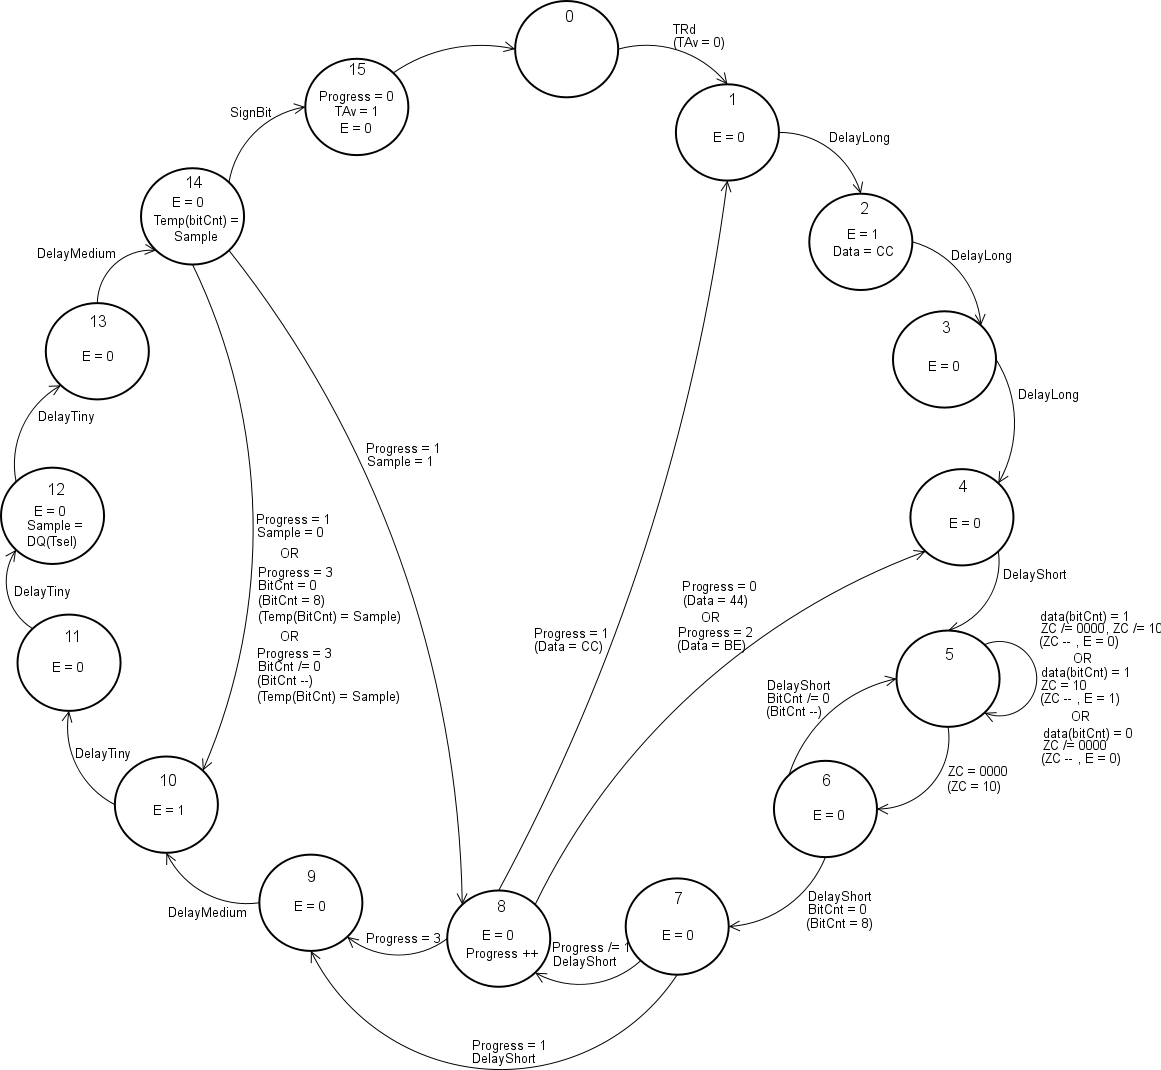
\includegraphics[scale=0.4, angle=0]{TempStateMachineDiagram.png}
	  	\caption{Detaljerat State Machine-diagram för Temperaturläscykel}
	\end{figure}

		\subsubsection{MT8880}
		\subsubsection{ISD2560P}

\section{Tidsdiagram}

	\begin{figure}[h!tb]
	  \centering
	      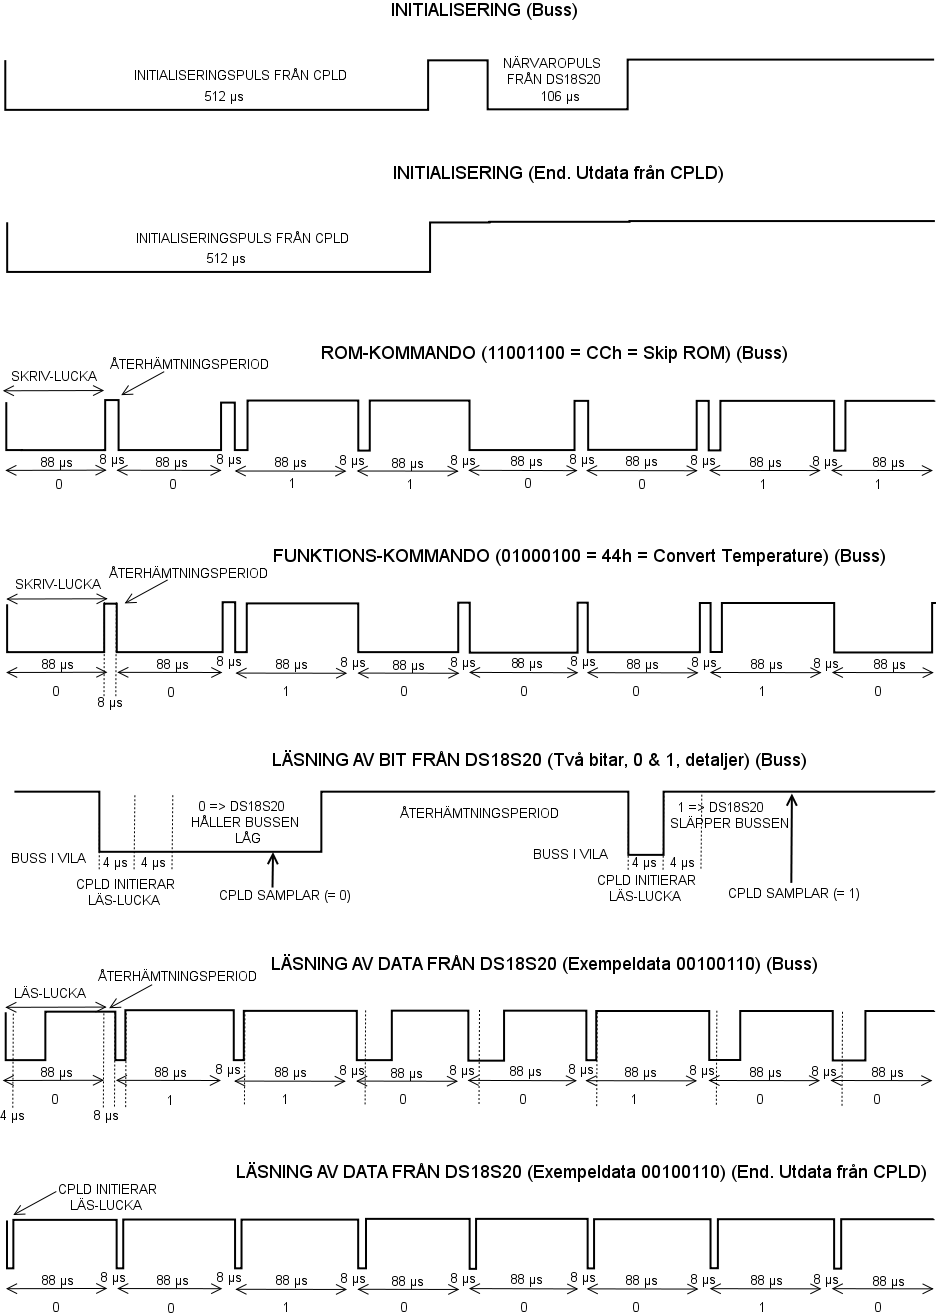
\includegraphics[scale=0.5, angle=0]{TempTiming.png}
	  	\caption{Timingdiagram för Temperaturmodulen}
	\end{figure}

\section{Felanalys}

\section{Appendix}

	\subsection{Komponentlista}
	\begin{tabular}{l r}
		\\{\bf Namn} & {\bf Beskrivning}\\
		XC9572XL (x2) & CPLD\\
		DS18S20 (x2) & Temperatursensor\\
		MT8880C & DTMF Transceiver\\
		ISD2560P & Ljudlagringskrets\\\\
	\end{tabular}

	\subsection{Kretsschema}

	\subsection{PCB-Schema}

	\subsection{Programlistningar}

	\subsection{Signallista}

\end{document}
